\documentclass[a4paper, 10pt]{article}
% (1) Encoding, Fonts, and Layout
\usepackage[T1]{fontenc}
\usepackage{lmodern}
\usepackage[margin=1in]{geometry}


% (2) Common Packages
\usepackage{amsmath, amssymb, amsthm}
\usepackage{xcolor}
\usepackage{caption}
\usepackage{tikz}
\usepackage{pgfplots}
\pgfplotsset{compat=newest}
\usepackage{etoolbox}
\usepackage{tikz-3dplot}
\tdplotsetmaincoords{75}{120}
\usepackage[inline]{enumitem}
\usepackage{bookmark}
\usepackage{mathtools}
\usepackage{subcaption} % For subfigures
\usepackage[normalem]{ulem} % For better underline commands

% Micro-typography
\usepackage{microtype}

% Patching pgfplots warning
\makeatletter
\patchcmd{\pgfplots@applistXXpushback@smallbuf}{\pgfplots@error}{\pgfplots@warning}{}{}
\makeatother

% (3) tcolorbox and Theorem Libraries
\usepackage{tcolorbox}
\tcbuselibrary{theorems}

% (4) Define Colors
\definecolor{custom_green}{HTML}{a3be8c}
\definecolor{custom_red}{HTML}{dc322f}
\definecolor{custom_blue}{HTML}{268bd2}
\definecolor{custom_purple}{HTML}{b48ead}

\definecolor{base}{HTML}{eceff4}
\definecolor{gray1}{HTML}{e5e9f0}
\definecolor{gray2}{HTML}{d8dee9}
\definecolor{gray3}{HTML}{2e3440}
\pagecolor{base}

% (5) Custom tcolorbox Environments
\newtcolorbox{definitionbox}[1][]{
    title=\textbf{Definition} {#1},
    fonttitle=\bfseries\boldmath,
    arc=0mm,
    bottomtitle=0.5mm,
    boxrule=0mm,
    colbacktitle=gray2,
    colback=gray1,
    coltitle=gray3,
    coltext=gray3,
    left=2.5mm,
    leftrule=1mm,
    rightrule=1mm,
    right=3.5mm,
    toptitle=0.75mm,
    colframe=custom_red,
}

\newtcolorbox{proofbox}{
    title=\textbf{Proof},
    fonttitle=\bfseries\boldmath,
    arc=0mm,
    bottomtitle=0.5mm,
    boxrule=0mm,
    colbacktitle=gray2,
    colback=gray1,
    coltitle=gray3,
    left=2.5mm,
    leftrule=1mm,
    rightrule=1mm,
    right=3.5mm,
    toptitle=0.75mm,
    colframe=custom_blue,
    coltext=gray3,
}

\newtcolorbox{theorembox}[1][]{
    title=\textbf{Theorem} {#1},
    fonttitle=\bfseries\boldmath,
    arc=0mm,
    bottomtitle=0.5mm,
    boxrule=0mm,
    colbacktitle=gray2,
    colback=gray1,
    coltitle=gray3,
    left=2.5mm,
    leftrule=1mm,
    rightrule=1mm,
    right=3.5mm,
    toptitle=0.75mm,
    colframe=custom_green,
    coltext=gray3
}

\newtcolorbox{notebox}{
    title=\textbf{Note},
    fonttitle=\bfseries\boldmath,
    arc=0mm,
    bottomtitle=0.5mm,
    boxrule=0mm,
    colbacktitle=gray2,
    coltitle=gray3,
    left=2.5mm,
    leftrule=1mm,
    rightrule=1mm,
    right=3.5mm,
    toptitle=0.75mm,
    colframe=custom_blue,
    coltext=gray3
}

\newtcolorbox{examplebox}[1][]{
    title=\textbf{Example} {#1},
    fonttitle=\bfseries\boldmath,
    arc=0mm,
    bottomtitle=0.5mm,
    boxrule=0mm,
    colbacktitle=gray2,
    colback=gray1,
    coltitle=gray3,
    left=2.5mm,
    leftrule=1mm,
    rightrule=1mm,
    right=3.5mm,
    toptitle=0.75mm,
    colframe=gray3,
    fontupper=\footnotesize,
    coltext=gray3
}

% (6) Theorem Environments
\theoremstyle{definition}
\newtheorem{definition}{Definition}[section]
\newtheorem{example}[definition]{Example}

\theoremstyle{plain}
\newtheorem{theorem}[definition]{Theorem}

% (7) Hyperlinks
\usepackage{hyperref}
\hypersetup{
    colorlinks=true,    % Use colored text for links
    linkcolor=custom_red,      % Set link text color to red
    pdfborder={0 0 0}   % Remove the default box around links
}

% macros.tex
\newcommand{\intinf}{\int_0^{\infty}} % Integral from 0 to infinity
\newcommand{\diff}[2]{\frac{d#1}{d#2}} % Derivative

\usepackage{listings}
\usepackage[hypcap=false]{caption}
\usepackage{algorithm}
\usepackage{algpseudocode}

\definecolor{commentgreen}{rgb}{0,0.5,0}
\definecolor{keywordsblue}{rgb}{0,0,0.8}
\definecolor{stringspurple}{rgb}{0.58,0,0.82}


\title{
\textbf{CS211: Programing For Operating Systems} \\ 
}

\author{
Robert Davidson
}     
\date{}       

\begin{document}

\maketitle
\pagebreak

\tableofcontents
\pagebreak
\subsection*{Useful headers}
\begin{itemize}
    \item \texttt{stdio.h} : Standard input/output library
    \item \texttt{stdlib.h} : Standard library
    \item  \texttt{string.h} : String manipulation functions (\texttt{strncpy, strcat, strcmp, strstr, strlen})
    \item \texttt{unistd.h} : Standard library for system calls (\texttt{fork, getpid, getppid})
\end{itemize}




\pagebreak
\subsection{Intro to C}

It is a very small language and relies heavily on libraries
The compiler must be told in advance how these functions should be used. So before the compilation process, the \textbf{preprocessor} is run to include the function prototypes The compiler then compiles the code into an object file.

\subsection{Hello World}
\begin{lstlisting}[style=cStyle, caption={Hello World in C}]
    #include <stdio.h>
    int main(){
        printf("Hello World\n");
        return 0;
    }
    \end{lstlisting}
\begin{itemize}
    \item \textbf{Line 1} : \texttt{\#include <stdio.h>} is a preprocessor directive that tells the compiler to include the standard input/output library. This library contains the \texttt{printf} function.
    \item In C almost every line it either preprocessor directive, variable declaration, or a function call.
    \item C uses curly braces to delimit blocks of code and semicolons to terminate statements.
    \item \textbf{Line 4}: In our case, we assume main is called by the Operating System, so return 0 is used to indicate that the program has run successfully.
\end{itemize}

\subsection{Variables}
In C all variables must be declared before they are used. The declaration should have a type; telling the compiler what sort of data the variable will hold. The types of variables are:
\begin{itemize}
    \item \textbf{int} : Integer (1, 2, 3, 4, 5, ...)
    \item \textbf{float} : Floating-point number (7 decimal digits)
    \item \textbf{double} : Double-precision floating-point number (15 decimal digits)
    \item \textbf{char} : Character (a, b, c, ...)
    \item \textbf{void} : No type  (used for functions that do not return a value)
\end{itemize}

We can Also declare arrays as follows:
\begin{lstlisting}[style=cStyle, caption={Declaring Arrays}]
    int arr[5]; // Array of 5 integers
    char name[10]; // Array of 10 characters
\end{lstlisting}
To access the first element of arr we can do \texttt{arr[0]}
\subsection{An Example}
\begin{lstlisting}[style=cStyle, caption={Example of Variables}]
    int d=-101;
    float f=1.23456;
    char c='a';
    printf("Values of d, f, c are: %d, %f, %c\n", d, f ,c );
\end{lstlisting}
\textbf{Explanation:} In this case, \texttt{\%d} is a placeholder for an integer, \texttt{\%f} is a placeholder for a float, and \texttt{\%c} is a placeholder for a character.

\subsection{Operators}

\begin{minipage}{0.45\textwidth}
    \centering
    \begin{tabular}{|c|c|c|}
        \hline
        Operator & Description    & Example         \\
        \hline
        +        & Addition       & \texttt{a + b}  \\
        \hline
        -        & Subtraction    & \texttt{a - b}  \\
        \hline
        *        & Multiplication & \texttt{a * b}  \\
        \hline
        /        & Division       & \texttt{a / b}  \\
        \hline
        \%       & Modulus        & \texttt{a \% b} \\
        \hline
    \end{tabular}
    \captionof{table}{Arithmetic Operators}
\end{minipage}
\hfill
\begin{minipage}{0.50\textwidth}
    \centering
    \begin{tabular}{|c|c|c|}
        \hline
        Operator & Description         & Example          \\
        \hline
        =        & Assignment          & \texttt{a = b}   \\
        \hline
        +=       & Add and assign      & \texttt{a += b}  \\
        \hline
        -=       & Subtract and assign & \texttt{a -= b}  \\
        \hline
        *=       & Multiply and assign & \texttt{a *= b}  \\
        \hline
        /=       & Divide and assign   & \texttt{a /= b}  \\
        \hline
        \%=      & Modulus and assign  & \texttt{a \%= b} \\
        \hline
        ++       & Increment           & \texttt{a++}     \\
        \hline
        --       & Decrement           & \texttt{a--}     \\
        \hline
    \end{tabular}
    \captionof{table}{Assignment and Arithmetic Assignment Operators}
\end{minipage}

\vspace{1em}
\begin{minipage}{0.50\textwidth}
    \centering
    \begin{tabular}{|c|c|c|}
        \hline
        Operator & Description      & Example         \\
        \hline
        ==       & Equal            & \texttt{a == b} \\
        \hline
        !=       & Not Equal        & \texttt{a != b} \\
        \hline
        >        & Greater          & \texttt{a > b}  \\
        \hline
        <        & Less             & \texttt{a < b}  \\
        \hline
        >=       & Greater or Equal & \texttt{a >= b} \\
        \hline
        <=       & Less or Equal    & \texttt{a <= b} \\
        \hline
    \end{tabular}
    \captionof{table}{Relational Operators}
\end{minipage}
\hfill
\begin{minipage}{0.45\textwidth}
    \centering
    \begin{tabular}{|c|c|c|}
        \hline
        Operator & Description & Example           \\
        \hline
        \&\&     & Logical AND & \texttt{a \&\& b} \\
        \hline
        ||       & Logical OR  & \texttt{a || b}   \\
        \hline
        !        & Logical NOT & \texttt{!a}       \\
        \hline
    \end{tabular}
    \captionof{table}{Logical Operators}
\end{minipage}





\subsection{Control Structure}
\begin{lstlisting}[style=cStyle, caption={If-Else}]
    int a = 10;
    if(a > 10){
            printf("a is greater than 10\n");
        }else if(a == 10){
            printf("a is equal to 10\n");
        }else{
    printf("a is less than 10\n");
    }
    \end{lstlisting}
Logical opeators, \texttt{\&\&} and \texttt{||} can be used to make more complex conditions.
\begin{lstlisting}[style=cStyle, caption={Complex If-Else}]
    if(a > 10 && a < 20){
        printf("a is between 10 and 20\n");
    }
    \end{lstlisting}
\subsubsection{For loop}
\texttt{for(initial val; continuation condition; increment/decrement)\{...\}}

\begin{lstlisting}[style=cStyle, caption={Print numbers from 0 to 9}]
for(int i = 0; i < 10; i++){
    printf("i is %d\n", i);
}
\end{lstlisting}
\pagebreak
\subsubsection{While loop}
\texttt{while(expression)\{...\}}
\begin{lstlisting}[style=cStyle, caption={Print numbers from 0 to 9}]
int i = 0;
while(i < 10){
    printf("i is %d\n", i);
    i++;
}
\end{lstlisting}
\subsubsection{Do While loop}
\texttt{do\{...\}while(expression);}
\begin{lstlisting}[style=cStyle, caption={Print numbers from 0 to 9}]
int i = 0;
do{
    printf("i is %d\n", i);
    i++;
}while(i < 10);
\end{lstlisting}

\subsection{Output}
\texttt{printf()} is used to print formatted output to the screen. It is a variadic function, meaning it can take any number of arguments. The first argument is a format string, followed by the values to be printed.\\[2ex]
The format string may contain a number of escape characters, represented by a backslash. Some of the most common escape characters are:
\begin{center}
    \begin{tabular}{|c|c|}
        \hline
        Sequence                               & Description                                  \\
        \hline
        \texttt{\textbackslash a}              & Produces a beep or flash                     \\
        \hline
        \texttt{\textbackslash b}              & Moves cursor to last column of previous line \\
        \hline
        \texttt{\textbackslash f}              & Moves cursor to start of next page           \\
        \hline
        \texttt{\textbackslash n}              & New line                                     \\
        \hline
        \texttt{\textbackslash r}              & Carriage return                              \\
        \hline
        \texttt{\textbackslash t}              & Tab                                          \\
        \hline
        \texttt{\textbackslash v}              & Vertical tab                                 \\
        \hline
        \texttt{\textbackslash \textbackslash} & Prints a backslash                           \\
        \hline
        \texttt{\textbackslash '}              & Prints a single quote                        \\
        \hline
    \end{tabular}
\end{center}
A conversion character is a letter that follows a \texttt{\%} and tells \texttt{printf()} to display the value stored in the corresponding variable. Some of the most common conversion characters are:
\begin{center}
    \begin{tabular}{|l|l|}
        \hline
        Specifier                    & Description                                  \\
        \hline
        \texttt{\%c}                 & Single character (char)                      \\
        \hline
        \texttt{\%d} or \texttt{\%i} & Decimal integer (int)                        \\
        \hline
        \texttt{\%e} or \texttt{\%E} & Floating-point (scientific notation)         \\
        \hline
        \texttt{\%f}                 & Floating-point value (float)                 \\
        \hline
        \texttt{\%g} or \texttt{\%G} & Same as \%e/\%E or \%f, whichever is shorter \\
        \hline
        \texttt{\%s}                 & String (char array)                          \\
        \hline
        \texttt{\%u}                 & Unsigned int                                 \\
        \hline
        \texttt{\%x}                 & Hexadecimal integer                          \\
        \hline
        \texttt{\%p}                 & Pointer (memory address)                     \\
        \hline
        \texttt{\%\%}                & Prints the \% character                      \\
        \hline
    \end{tabular}
\end{center}
\pagebreak
\subsection{Input}
\texttt{scanf()} reads input from standat input, format it, as directed by a conversion character and store the address of a specified variable.
\begin{lstlisting}[style=cStyle, caption={Reading an integer}]
    int number; 
    char letter; 
    printf("Enter a number and a char: ");
    scanf("%d %c", &number, &letter);

    printf("You entered: %d and %c\n", number, letter);
\end{lstlisting}
\begin{itemize}
    \item The scan \texttt{scanf()} returns an integer equal to the number of successfull conversions made.
    \item There is related function \texttt{fscanf()} that reads from a file. \texttt{scanf()} is really just a wrapper for \texttt{fscanf()} that treats the keyboard as a file.
    \item There are other useful functions for readint the standard input stream: \texttt{getchar()} and \texttt{gets()}.
\end{itemize}
\begin{lstlisting}[style=cStyle, caption={Check for no input}]
    int number;
    printf("Enter a number between 1 and 30: ");
    scanf("%d", &number);

    while ((number<1) || (number>30))
    {
        printf("Invalid number. Please enter a number between 1 and 30: ");
        scanf("%d", &number);
    }
\end{lstlisting}

\subsection{Functions}
\begin{definitionbox}{Protype and Definition}{}
    A \textbf{Protype :} A function prototype is a declaration of a function that tells the compiler what the function looks like. It includes the function name, return type, and parameter types. The prototype must be declared before the function is called. \\
    \textbf{Definition :} A function definition is the actual implementation of the function. It includes the function name, return type, parameter types, and the body of the function. The definition must be declared after the function is called.
\end{definitionbox}

\subsection{Call-by-Value and Pointers}
In C is it important to distuinguish between a variable and the value stored in it. A variable has a location in memory. The value of the variable is stored in that location. For example:
\begin{lstlisting}[style=cStyle]
int i = 10;
\end{lstlisting}
tells the system to allocate a location in memory to store the value 10. The variable \texttt{i} is a pointer to that location in memory. One of the distuinguihing features of C is it we can manipulate the memory address of the variable almost as easily as we can manipulate the value stored in it.
\begin{conceptbox}{Pointers}{}
    \begin{itemize}
        \item if \texttt{i} is a variable, then \texttt{\&i} is a pointer to the location in memory where the value of \texttt{i} is stored.
              If a memory address is stored in the variable \texttt{p}, then \texttt{*p} is the value stored at that address.
        \item If a memory address is stored in the variable \texttt{p}, then \texttt{*p} is the value stored at that address.
    \end{itemize}
\end{conceptbox}
\pagebreak
\subsection{Characters}
\begin{conceptbox}{Character representation}{}
    In C, a character is just an unsigned integer. Each character is represented by an integer between 0 and 127.
\end{conceptbox}

\begin{minipage}{0.45\textwidth}
    \textbf{Printing characters:}

    \begin{itemize}
        \item \texttt{printf("\&c", c)}
        \item \texttt{putchar(c)}
    \end{itemize}
\end{minipage}
\begin{minipage}{0.45\textwidth}
    \textbf{Reading characters:}
    \begin{itemize}
        \item \texttt{scanf("\&c", c)}
        \item \texttt{c = getchar()}
    \end{itemize}
\end{minipage}
\subsection{Strings}
\begin{conceptbox}{String representation}{}
    C does not have a string data type. Instead it uses arrays of type char to represent strings. For example if we make a declaration:
    $$\texttt{char greeting[20]="Hello. How are you?";}$$
    the system stores each character as an element of the array greeting.
\end{conceptbox}
\subsubsection{String Functions}
Useful functions defined in \texttt{string.h}: \\[2ex]
$$\texttt{char *strncp(char *dest, char *src, int n)} $$
Copies at most \texttt{n} characters from \texttt{src} to \texttt{dest}. The advantage of this is that we don't copy more chatavyers to \texttt{dest} than it can hold (prevents buffer overflow). \texttt{strncpy()} does not append a null character to the end of the string, so we need to do that manually. \\[2ex]
$$\texttt{char *strcat(char *dest, char *src)}$$
Concatenates the string \texttt{src} to the end of the string \texttt{dest}. The destination string must be large enough to hold the concatenated result. \texttt{strcat()} appends a null character to the end of the string. \\[2ex]
$$\texttt{int strcmp(char *str1, char *str2)}$$
Compares two strings annd returns an intger:
\begin{itemize}
    \item 0 if the strings are equal
    \item A negative integer if \texttt{str1} comes first alphabetically
    \item A negative integer if \texttt{str2} comes first alphabetically
\end{itemize}
$$\texttt{char *strstr(char *haystack, char *needle)} $$
Searches for the first occurrence of the string \texttt{needle} in the string \texttt{haystack}. If found, it returns a pointer to the first occurrence of \texttt{needle} in \texttt{haystack}. If not found, it returns NULL. \\[2ex]
$$\texttt{int strlen(char *str)}$$
Returns the length of the string \texttt{str} (not including the null character).

\pagebreak
\subsection*{1.11 Strings (Continued)}
\subsubsection{String Output}
We know how to use \texttt{printf()} to print strings:
\begin{itemize}
    \item \texttt{printf("\%s\%s$\backslash$n, "Good Morning ", name);}
    \item \texttt{printf("\%s\%8s$\backslash$n", "Good Morning ", name);}
\end{itemize}
The second example, the field width specifier is given. This causes the string to be padded so it takes up a total of 8 spaces. If the string is shorter than 8 characters, it is padded with spaces on the left. If the string is longer than 8 characters, it is printed as is.

\subsubsection{String Input}
\begin{itemize}
    \item \texttt{scanf("\%s", name);} reads the next "word" from th input stream and stores it in the array \texttt{name}. A "word" is defined as a sequence of characters separated without a space, tab, or newline. The string is terminated with a null character.
    \item \texttt{getchar(name);} to get more control of the input in a loop
    \item \texttt{gets(string);} reads a line input and stores it all except the newline character. The string is terminated with a null character. \texttt{gets()} is not safe to use because it does not check the length of the input string. If the input string is longer than the array, it will cause a buffer overflow and overwrite other data in memory.
    \item \texttt{fgets(string, n, stdin);} reads in a line of text from the keyboard (standard input stream) and stores at most \texttt{n} characters in the array \texttt{string}. The string is terminated with a null character. If the input string is longer than \texttt{n}, it will be truncated and the rest will be discarded. \texttt{fgets()} is safer to use than \texttt{gets()} because it checks the length of the input string.
\end{itemize}
\subsection{Arrays}
\subsection{Arrays}
To declare a $3 \times 4$ matrix of floats, we write \texttt{float a[3][4];}. So:
$$\begin{bmatrix}
        a[0][0] & a[0][1] & a[0][2] & a[0][3] \\
        a[1][0] & a[1][1] & a[1][2] & a[1][3] \\
        a[2][0] & a[2][1] & a[2][2] & a[2][3]
    \end{bmatrix}
$$
In general, an $n \times m$ array is declared as \texttt{float a[n][m];}. The first index is the row number and the second index is the column number. The first element of the array is \texttt{a[0][0]} and the last element is \texttt{a[n-1][m-1]}. \\[2ex]
If a has the line \texttt{int [a][4];} then the system creats three arrays, each of length four. More precisely, it:
\begin{itemize}
    \item declares 3 pointers to type \texttt{int}: \texttt{a[0]}, \texttt{a[1]}, and \texttt{a[2]}
    \item space for storing an integer is allocated to each of addresses \texttt{a[0], a[0]+1, a[0]+2, a[0]+3, a[1], a[1]+1}, $\dots$, \texttt{a[2]+3}
\end{itemize}
This mean is if \texttt{a[][]} is declared as a two-dimensional $3 \times 4$ array, then the following are equivalent:
\begin{itemize}
    \item \texttt{a[1][2]}
    \item \texttt{*(a[1]+2)}
    \item \texttt{*(*(a+1)+2)}
    \item \texttt{*(\&a[0][0]+4+2)}
\end{itemize}
\pagebreak
\subsection{Explanation of Array Element Access in C}

\subsubsection*{\texttt{a[1][2]}}
This is the standard way to access a two-dimensional array element. It directly fetches the element in the second row (index 1) and the third column (index 2).

\subsubsection*{\texttt{*(a[1]+2)}}
\begin{itemize}
    \item \texttt{a[1]} yields the second row, which decays to a pointer to its first element (i.e., equivalent to \texttt{\&a[1][0]}).
    \item Adding \texttt{2} moves the pointer two elements forward in that row.
    \item The dereference operator \texttt{*} then accesses the element at that position, which is \texttt{a[1][2]}.
\end{itemize}

\subsubsection*{\texttt{*(*(a+1)+2)}}
\begin{itemize}
    \item \texttt{a+1} moves the pointer from the first row to the second row.
    \item \texttt{*(a+1)} dereferences that pointer to yield the address of the first element of the second row (again, equivalent to \texttt{a[1]}).
    \item Adding \texttt{2} moves to the third element in that row, and the outer \texttt{*} fetches its value \rule{\textwidth}{0.5pt}again, \texttt{a[1][2]}.
\end{itemize}

\subsubsection*{\texttt{*(\&a[0][0]+4+2)}}
\begin{itemize}
    \item \texttt{\&a[0][0]} gets the address of the very first element of the array.
    \item Since the array is stored in contiguous memory, pointer arithmetic treats it as a flat sequence. Adding \texttt{4+2} (i.e., 6) moves the pointer to the 7th element in that sequence.
    \item If the layout of the array is such that the element \texttt{a[1][2]} is the 7th element (this is true, for example, if the row length is at least 3), then dereferencing this pointer retrieves \texttt{a[1][2]}.
\end{itemize}

\subsection{Files}
Taking an input from a file is not much different than taking input from a keyboard. All we do is:
\begin{itemize}
    \item Declare an identifier of type \texttt{FILE} to hold the file pointer.
    \item Open the file (\texttt{fopen()})
    \item Read the file
    \item Close the file (\texttt{fclose()})
\end{itemize}
\subsection{Declaring a file indentifier:}
$$\texttt{FILE *datafile;}$$
The datafile is now a pointer we can associate with a file. The \texttt{FILE} type is defined in the \texttt{stdio.h} library.
\subsection{Opening a file:}
$$\texttt{fileptr = fopen(char *filename, char *mode);}$$
The \texttt{fopen()} is a function that is use for file opening. It takes two arguments: the name of a file and the mode it will operrate in. A file pointer is returned. The mode can be:
\begin{itemize}
    \item \texttt{r} : read (open an existing file for reading)
    \item \texttt{w} : write (overrwite the file or create a new one)
    \item \texttt{a} : append (add to the end of the file)
\end{itemize}
\subsection{Closing a File}
$$\texttt{fclose(fileptr);}$$
Once a file is “closed” we can no longer read from it or write to it, unless
we open it again. If we don't do this, the file will still be closed when the
program terminates. But until then, no other program on the same node
(computer) can work with the file, and it might but be fully written to
storage
\subsection{Reading from a file}
$$\texttt{fgets(char *str, int n, FILE *fileptr);}$$
reads in a line of text from the fileptr stream and stores at most n
characters in array sting. The mew line character is stored.
If the string can't be read, because we have reached the end of the file,
then NULL is returned.
$$\texttt{fgetc(FILE *fileptr);}$$
reads the next character in the file and stores it in the char variable c. If
the end of the file has been reached, EOF is returned.
$$\texttt{fscanf(FILE *fileptr, char *format, ...);}$$
reads formatted input from the file. The format string is similar to the
one used in \texttt{printf()}
\subsection{Navigating a file}
Each time a character is reader from the input stream, a counter associated with the stream is incremented.
$$\texttt{rewind(FILE *fileptr);}$$
sets the indicator to the start of the file
$$\texttt{ftell(FILE *fileptr);}$$
is used to check the current value of the file position indivator in the form of a long int.
$$\texttt{fseek(FILE *fileptr, long offset, int place);}$$
the value of offset is the amount the indicator will be changed by, while placce is one of:
\begin{itemize}
    \item \texttt{SEEK\_SET(0)} : the start of the file
    \item \texttt{SEEK\_CUR(1)} : the current position in the file
    \item \texttt{SEEK\_END(2)} : the end of the file
\end{itemize}
\subsection{Writing to a file}
To write to a file, we declare a file pointer:
$$\texttt{FILE *outfile;}$$
and open a new file in write mode:
$$\texttt{outfile = fopen("myList.txt", "w");}$$
to write to the file, we use one of:
\begin{itemize}
    \item \texttt{fprintf(outfile, char *format, ...);} : works like \texttt{printf()} except its first argument is a file pointer
    \item \texttt{fputs(char *str, FILE *fileptr);} : writes the string str to the file pointed to by fileptr, without its trailing '\texttt{\textbackslash 0}' character. The string is not formatted.
    \item \texttt{fputc(int c, FILE *fileptr);} : writes the character c to the file pointed to by fileptr. The character is not formatted.
\end{itemize}
\pagebreak
\subsection{Issues concerining the use of files in C, we should be aware of:}
\begin{itemize}
    \item There are 6 modes a file can have: \texttt{r, w, a, r+, w+, a+}
    \item To open a binary file, also add a \texttt{b} to the mode. For example, \texttt{rb} opens a file for reading in binary mode.
    \item \texttt{freopen()} attaches a new file to an existing file pointer. It is used to redirect the standard input or output to a file. For example, \texttt{freopen("myList.txt", "w", stdout);} redirects the standard output to the file \texttt{myList.txt}. This means that any output that would normally go to the screen will now go to the file.
    \item \texttt{tmpfile()} open a tempory file in binary read/write and is automatically deleted when closed or when the program terminates
    \item \texttt{fflush(fileptr);} flushes the output buffer of the file pointer. This means that any data that has been buffered but not yet written to the file will be written to the file.
    \item \texttt{remove("myList.txt");} deletes the file \texttt{myList.txt} from the disk.
    \item \texttt{rename("myList.txt", "myList2.txt");} renames the file \texttt{myList.txt} to \texttt{myList2.txt}. If the new name already exists, it will be overwritten.
    \item \texttt{int feof(FILE *fileptr);} returns a non-zero value if the end of the file has been reached. It is used to check if we have reached the end of the file while reading it.
\end{itemize}

\subsection{The Process}
$$\textbf{"A process is a running program."}$$
The operating system gives the impression many programs are running at the same time, but in reality, only one program is running at a time. This is made possible by abstracting the the concept of a running program as a process.
\begin{conceptbox}{Every process has}{}
    \begin{itemize}
        \item \textbf{The process text:} the program code
        \item \textbf{The program counter:} the address of the next instruction to be executed
        \item \textbf{The process stack:}  temporary data, local variables, function parameters, return addresses
        \item \textbf{The data section:}  global variables
    \end{itemize}
\end{conceptbox}
A process is not just a program - if two users run the same program at the same time, they create different processes. Each process has its own memory space, so they do not interfere with each other. A program is a passive entity, while a process is an active / dynamic entity.
\begin{conceptbox}{Operations OS must perform on a process}{}
    \begin{itemize}
        \item \textbf{Create} a new process (open a new program)
        \item \textbf{Terminate / Destory} a process (close a program)
        \item \textbf{Wait} or pause a process until some event occurs (e.g. waiting for user input)
        \item \textbf{Supsend and Resume} similar to wait but more explicit
        \item \textbf{Status}  report info about a process (e.g. how much memory it is using, how long it has been running, etc.)
    \end{itemize}
\end{conceptbox}
\begin{conceptbox}{States of a process}{}
    \begin{itemize}
        \item \textbf{New} : the process is being created
        \item \textbf{Running} : instructions being executed
        \item \textbf{Block / Waiting} : waiting for some event to occur (e.g. I/O operation)
        \item \textbf{Ready} : waiting to be assigned to a processor
        \item \textbf{Terminated} : the process has finished executing
    \end{itemize}
\end{conceptbox}

\pagebreak
\subsection{Process Creation}
A parent creates a child process. The child process can create its own child, forming a tree of processes. After a parent creates a child process it may:
\begin{itemize}
    \item \textbf{Execute} concurrently with the child process
    \item \textbf{Wait} until the child process terminates to continue
\end{itemize}
The parent may share all, none or some of its resources with the child process (memory space, open files, etc.)
\subsection{Process Identifcation Number}
ll processes have a unique identifier called a \textbf{PID}. If we create a child process in C, using a \texttt{fork()} a new process is created:
\begin{itemize}
    \item The new process runs \textbf{concurrently} with the parent, unless we instruct it to \texttt{wait()}.
    \item The subproc (child) is given a \textbf{copy of the parents memory space}
    \item At the time of creation, the two processes are identical, except the \texttt{fork()} returns te child process' PID to the parent and 0 to the child.
\end{itemize}
In order to use \texttt{fork()} , we must include the \texttt{unistd.h} library, which includes:
\begin{itemize}
    \item \texttt{fork()} - creates a new process
    \item \texttt{getpid()} - returns the PID of the calling process
    \item \texttt{getppid()} - returns the PID of the parent process
\end{itemize}
\subsubsection{\texttt{unistd.h} functions}
$$\boxed{\texttt{pid\_t fork(void);}}$$
\begin{itemize}
    \item It takes no arguments
    \item It returns an \texttt{int}
    \item It returns -1 if the fork failed
    \item Otherwise, it returns the PID of the newly created child process to the parent process
    \item It returns 0 to the child process
    \item The child process is distinct from the parent (it gets its own copy of the parent's memory space)
    \item Both parent and child process run concurrently
    \item Starting from the \texttt{fork()} call, the parent and child process execute the same instruction set.
\end{itemize}
$$\boxed{\texttt{pid\_t getpid(void);}}$$
Returns the value of the processes own PID
$$\boxed{\texttt{pid\_t getppid(void);}}$$
Returns the value of the parent process' PID
Since the parent and subproc (child) have copies of the same memory space and instruction set, \texttt{getpid()}  and \texttt{getppid()} are useful for working out which is which.
\pagebreak
\subsection{Process Programming}
Often we don't want the parent to continue running while the child is running, the results may be non-deterministic. Recall a sub-proc will share the parents memory only in a sense that it recieves a copy. The  child process can mimic the parents execution  or its memory space may be overlaid with a new program/set of instructions. \\[2ex]

Often when a child process is created it is overlaid with another program. In C, this can be done with the {exelclp()} function. In the following example, the sub-procs memory space is overlaid the program text of the ls command.  Again we will use the \texttt{wait()} function.\\[2ex]
The OS is responsible for \textbf{de-allocating the resources} of a process that has finished. It may also be responsible for terminating a process that is not responding.
\begin{conceptbox}{Processes are terminated when}{}
    \begin{itemize}
        \item The proc executes its last instruction and asks the operating system to delete it (\texttt{exit()}). At that time it will usualy:
              \begin{itemize}
                  \item Output data from subproc to parent (via \texttt{wait()})
                  \item Have its resources de-allocated by the OS
              \end{itemize}
        \item Parent terminates a child process because:
              \begin{itemize}
                  \item Sub-proc has exceeded allocated resources
                  \item The task assigned to the sub-proc is no longer needed
              \end{itemize}
        \item The parent is exiting and the OS does not allow subproc to continue if the parent is terminated
    \end{itemize}
\end{conceptbox}
\subsection{Signals}
The \texttt{kill()} system call is an example of a signal - a form of communication from one process to another. These provide a facility for asynchronus event handling. Note - when the subproc sends the kill() signal to the parent, the subproc also terminates. \\[2ex]
The \texttt{kill()} function can send other signals, but most (such as SIGABRT, SIGILL, SIGQUIT, SIGTERM) are just variants of SIGKILL. However there are signals that preform other taks.
\begin{conceptbox}{Types of Signals}{}
    \begin{itemize}
        \item \textbf{SIGSTOP:} stops a process
        \item \textbf{SIGCONT:} continues a stopped process
        \item \textbf{SIGUSR1:} user defined signal 1
        \item \textbf{SIGUSR2:}  user defined signal 2
    \end{itemize}
\end{conceptbox}
The kill function can take two arguments:
$$\texttt{kill(pid\_t pid, int sig);}$$
the PID of the process to send the signal to and the signal to send. The function returns 0 on success and -1 on failure. The \texttt{kill()} function can be used to send any signal to any process, including itself. \\
With the \texttt{signal()} function, we can send a signal that tells the process to preform a specific asction, when it recieves a \texttt{SIGUSR1} or \texttt{SIGUSR2} signal.

\pagebreak

\subsection{Inter Process Communication}
Inter process communication (IPC) is a mechanism that allows processes to communicate with each other. This is important because processes may need to share data or synchronize their actions

\begin{conceptbox}{Types of Process Communication}{}
    \begin{itemize}
        \item \textbf{Independent} : Cannot affect or be affected by each other
        \item \textbf{Co-operating} : Can be affected by the execution of eachother
    \end{itemize}
\end{conceptbox}
\begin{conceptbox}{Why we allow IPC}{}
    \begin{itemize}
        \item \textbf{Information sharing} - two procs might require acess to the same file
        \item \textbf{Modularity} - Different procs might be dedicated to different system functions
        \item \textbf{Convenience} - a user might be running an editor, spell checker and printer all for the same file
        \item \textbf{Computational Speed} - on a multiprocessing system tasks are sub-divided and executred conrurrently on different processors.
    \end{itemize}
\end{conceptbox}

\begin{definitionbox}{Producer Consumer Model}{}
    One process (editor) has information it wants to produce for consumption by another (printer). This may be done by a \textbf{mutual/shared buffer}. Producer write to the buffer and consumer reads from it.
\end{definitionbox}
\begin{conceptbox}{Shared Buffer Types}{}
    \begin{itemize}
        \item \textbf{Un-bounded} : no size limit placed on the buffer. The producer may continue to produce and write to the buffer as long as it wants to.
        \item \textbf{Bounded} : strict size limit on the buffer. If full, producer must wait until consumer removes some data.
    \end{itemize}
\end{conceptbox}
\begin{conceptbox}{How we implement shared buffers}{}
    \begin{itemize}
        \item \textbf{Physically} by a set of shared variables (shared memory addresses), the implementation of this is the responsibility of the programmer.
        \item \textbf{Logically} by message passing using an Inter Process Communication. Such system is inplemented by the OS.. The IPC prodives a logical communcation link via a message passing facilitiy with two funadmental operations : \textbf{send message} and \textbf{recieve message}.
    \end{itemize}
\end{conceptbox}

\pagebreak
\subsubsection{Direct Communication}
Each process must nomiate the process they want to communicate it. Pairs of cumminicting processes must know each others ID's in order to etablish a link. With this system a link is established by the two processes automatically, there are exactly two processes in the link and there can be at most one link between two procss\\[2ex]
This is an example of \textbf{Symmetric addressing}. In the \textbf{Asymmetric addressing} model, the recipient listens out for any messages addressed to it (like making a phone call).\\[2ex]
\textbf{Disadvantages}
\begin{itemize}
    \item Processes must have details of eachother befoe they can communicate
    \item One link between processes only
    \item Only two processes can communicate at a time
\end{itemize}
\subsubsection{Indirect Communication}
The alternative is to have a number of ports (mailboxes) in the sytem. Each with a unique ID. \\[2ex]
For procs to communicae they must know the name of the mailbox. More than two procs can share a mailbox . Two procs may share more than one mailbox \\[2ex]
\textbf{Disadvantages}
\begin{itemize}
    \item Mailbox is owned by only one proc. Several procs can write to it, but only one can read from it.
    \item Procs are owned only by the OS. Permissions are then granted to processes to create and delete mailbox and to send and receive messages.
\end{itemize}
\subsection{\texttt{pipe()}}
A means of communication, based around the \texttt{pipe(), write(), read()} functions that allows one process to send data to another. The data can be anything, but we will use examples of sending integers. This is an example of \textbf{Symmetric direct communication}.

\subsection{Theads}
So far, we've assumed that every process has its own program counter (PC), which tells the OS where it is in its instruction set (think line of program currently executing). So even when we duplicate using \texttt{fork()} the new subproc has its own PC, even though they have the same value as the parents PC. \\[2ex]
However, modern OS's allow for threads: single process that can have mulitple PC's.

\begin{conceptbox}{Why threads are useful}{}
    \begin{itemize}
        \item The process may need to preform lots of operations at the same time (on different cores) on the same data - i.e. adding vectors
        \item Processes have to preform different operation that run at different speeds, such as adding vectors (fast) and waiting for user input (slow)
    \end{itemize}
\end{conceptbox}
But, with subprocs made with \texttt{fork()} memory is not really shared, so the advantage of being able to do things at once is lost by the need to communicate.
\pagebreak
\subsection{Single Point of Exuction vs Multiple Points of Execution}
Instead of our classic view of a single point of execution withing a program, a multi-threaded program has more than one point of execution. Each thread is very much like a seperate process, except for \textbf{one difference:} they share the same address and space and thus can acess the same data.
\begin{definitionbox}{Thread}{}
    A thread (or lightweight process) is a basic unit of CPU utilization. Rather than a process being dedicated to one sequential list of tasks it may be broken into threads. These consists a set of distinct:
    \begin{itemize}
        \item \textbf{Program Counter} - the next instruction to be executed
        \item \textbf{Register set} - operands for CPU instructions
        \item \textbf{Stack} - temporary variables, etc.
    \end{itemize}
\end{definitionbox}
\begin{definitionbox}{Task}{}
    A task is a collection of threads that belong to the same process and share code section, data section, and operating-system resources.
\end{definitionbox}
\begin{conceptbox}{Why use threads over processes}{}
    \begin{itemize}
        \item \textbf{Parallization} - Each thread can execute on a different processor core.
        \item \textbf{Responsiveness} - A part of a process may continue working, even if another part is blocked, i.e. waiting for an I/O operation
        \item \textbf{Resource Sharing} - For exampl we can have several hundred threads running at the same time. If they were all processes, we would have to allocate memory for each one. This is not the case with threads, as they share the same address space.
        \item \textbf{Economy} - Thread creation is faster than process creation and context switching is faster
        \item \textbf{Efficiency} - Threads belong to the same proc share common memory space and do not need support from the OS to communicate.
    \end{itemize}
\end{conceptbox}
\subsection{Two types of threads - User and Kernel}

On Linux, Mac and related systems, in C we can create threads called \texttt{pthreads} (POSIX threads) which are defined in the \texttt{pthread.h} header. We will use two functions:
\begin{itemize}
    \item \texttt{pthread\_create()} - used for creating thread and takes four arguments.
          \begin{itemize}
              \item ID of thread process
              \item Thread attributes (we'll ignore and use NULL)
              \item A function called by thread when created
              \item Argument to pass to the function.
          \end{itemize}
    \item \texttt{pthread\_join()} - tells parent to wait for a thread to finish
\end{itemize}

\begin{table}[h!]
    \centering
    \begin{tabularx}{\textwidth}{@{} l X X @{}}
        \toprule
        Thread Type    & User Threads                                                                                                  & Kernel Threads                                                                                                               \\
        \midrule
        Implementation & Implemented by a thread library at compiler/library level above the OS kernel                                 & Created, managed and scheduled by the operating system kernel                                                                \\
        Advantages     & Quick to create and destroy since system calls are not required                                               & Do not suffer from blocking problems; if one thread blocks, the kernel can schedule another thread from the same application \\
        Disadvantages  & If the kernel is not threaded and one thread makes a blocking system call, the entire process will be blocked & Slower to manipulate compared to user threads due to system call overhead                                                    \\
        \addlinespace[2ex]
        \bottomrule
    \end{tabularx}
\end{table}

\subsection{Sheduling Algorithms}
$$\textbf{"Several process/jobs are available to be run. In what order should they be executed?}$$
\subsection{Metrics to Compare Algoritms}
\begin{conceptbox}{Metrics to Compare Algorithms}{}
    \begin{itemize}
        \item \textbf{Turnaround time} - the total time taken to execute a process. It is the sum of the waiting time and the burst time.
        \item \textbf{Waiting time} - the total time a process has been waiting in the ready queue.
        \item \textbf{Response time} - the time taken from when a request was submitted until the first response is produced.
    \end{itemize}
\end{conceptbox}
\begin{table}[h!]
    \centering
    \begin{tabularx}{\textwidth}{@{} X X X @{}}
        \toprule
        Algorithm                & Advantages                                                                                                                    & Disadvantages \\
        \midrule
        FIFO (First In First Out)
                                 & Simple to implement, only need a FIFO queue. It is non-preemptive
                                 & Has a long average weight time, and suffers from the \textbf{convoy effect} (short jobs wait for long jobs)
        \\
        \addlinespace[2ex]
        SJF (Shortest Job First) & Optimal - minimum average waiting time for a given set of processes.
        Is non pre-eemptive.
                                 & Cannot be emplyed in a realisting setting because we would be required to know the length of next CPU Burst before it happens
        \\
        \addlinespace[2ex]
        STCF (Shortest Time to Completion First)
                                 & "More optimal” than SJF when processes arrive at
        different times
                                 & Needs preempting
        \\
        \addlinespace[2ex]
        RR (Round Robin)         & Fair, each process gets a fair share of the CPU. It is preemptive and simple to implement
                                 & Average waiting time is high, and it is not optimal for short jobs
    \end{tabularx}
\end{table}
\subsection{RR - Round Robin}
\begin{definitionbox}{Round Robin}{}
    A preemptive version of FIFO. Each process is assigned a time slice (quantum) and is executed for that time. If it does not finish, it is put back in the queue and the next process is executed.
\end{definitionbox}
\begin{examplebox}{}{}
    \scriptsize
    \begin{tabularx}{\textwidth}{@{} l X X @{}}
        \toprule
        Proc  & Arrival Time & Burst Time \\
        \midrule
        $P_1$ & 0            & 20         \\
        $P_2$ & 0            & 15         \\
        $P_3$ & 4            & 10         \\
        $P_4$ & 6            & 5          \\
    \end{tabularx}\\[2ex]
    \rule{\textwidth}{0.5pt}
    \textbf{1. First-Come, First-Served (FCFS)}

    \begin{minipage}[t]{0.48\textwidth}
        Order: $P_1 \rightarrow P_2 \rightarrow P_3 \rightarrow P_4$

        \begin{itemize}
            \item $P_1$: starts at 0, ends at 20
            \item $P_2$: starts at 20, ends at 35
            \item $P_3$: starts at 35, ends at 45
            \item $P_4$: starts at 45, ends at 50
        \end{itemize}

        \begin{align*}
            \text{TAT} & = \text{Completion Time} - \text{Arrival Time} \\
            \text{WT}  & = \text{TAT} - \text{Burst Time}               \\
            \text{RT}  & = \text{Start Time} - \text{Arrival Time}
        \end{align*}
    \end{minipage}
    \hfill
    \begin{minipage}[t]{0.48\textwidth}
        \begin{center}
            \begin{tabular}{@{} l c c c c @{}}
                \toprule
                Process & CT & TAT & WT & RT \\
                \midrule
                $P_1$   & 20 & 20  & 0  & 0  \\
                $P_2$   & 35 & 35  & 20 & 20 \\
                $P_3$   & 45 & 41  & 31 & 31 \\
                $P_4$   & 50 & 44  & 39 & 39 \\
                \bottomrule
            \end{tabular}
        \end{center}

        \begin{align*}
            \text{Average TAT} & = \frac{20 + 35 + 41 + 44}{4} = 35  \\
            \text{Average WT}  & = \frac{0 + 20 + 31 + 39}{4} = 22.5 \\
            \text{Average RT}  & = \frac{0 + 20 + 31 + 39}{4} = 22.5
        \end{align*}
    \end{minipage}

    \rule{\textwidth}{0.5pt}

    \textbf{2. Shortest Job First (SJF, Non-preemptive)}

    \begin{minipage}[t]{0.48\textwidth}
        \begin{itemize}
            \item At time 0: $P_1$, $P_2$ ready → pick $P_2$
            \item At time 15: $P_1$, $P_3$ ready → pick $P_3$
            \item At time 25: $P_1$, $P_4$ ready → pick $P_4$
            \item At time 30: $P_1$ runs
        \end{itemize}

        \begin{itemize}
            \item $P_2$: start 0, end 15
            \item $P_3$: start 15, end 25
            \item $P_4$: start 25, end 30
            \item $P_1$: start 30, end 50
        \end{itemize}
    \end{minipage}
    \hfill
    \begin{minipage}[t]{0.48\textwidth}
        \begin{center}
            \begin{tabular}{@{} l c c c c @{}}
                \toprule
                Process & CT & TAT & WT & RT \\
                \midrule
                $P_2$   & 15 & 15  & 0  & 0  \\
                $P_3$   & 25 & 21  & 11 & 11 \\
                $P_4$   & 30 & 24  & 19 & 19 \\
                $P_1$   & 50 & 50  & 30 & 30 \\
                \bottomrule
            \end{tabular}
        \end{center}

        \begin{align*}
            \text{Average TAT} & = \frac{15 + 21 + 24 + 50}{4} = 27.5 \\
            \text{Average WT}  & = \frac{0 + 11 + 19 + 30}{4} = 15    \\
            \text{Average RT}  & = \frac{0 + 11 + 19 + 30}{4} = 15
        \end{align*}
    \end{minipage}

    \rule{\textwidth}{0.5pt}

    \textbf{3. Round Robin (RR), Time Quantum = 10}

    \begin{minipage}[t]{0.48\textwidth}
        Execution sequence:
        \begin{itemize}
            \item 0-10: $P_1$ (rem 10)
            \item 10-20: $P_2$ (rem 5)
            \item 20-30: $P_3$ (done)
            \item 30-35: $P_4$ (done)
            \item 35-45: $P_1$ (done)
            \item 45-50: $P_2$ (done)
        \end{itemize}

        Response times:
        \begin{itemize}
            \item $P_1$: 0
            \item $P_2$: 10
            \item $P_3$: 20
            \item $P_4$: 30
        \end{itemize}
    \end{minipage}
    \hfill
    \begin{minipage}[t]{0.48\textwidth}
        \begin{center}
            \begin{tabular}{@{} l c c c c @{}}
                \toprule
                Process & CT & TAT & WT & RT \\
                \midrule
                $P_1$   & 45 & 45  & 25 & 0  \\
                $P_2$   & 50 & 50  & 35 & 10 \\
                $P_3$   & 30 & 26  & 16 & 20 \\
                $P_4$   & 35 & 29  & 24 & 30 \\
                \bottomrule
            \end{tabular}
        \end{center}

        \begin{align*}
            \text{Average TAT} & = \frac{45 + 50 + 26 + 29}{4} = 37.5 \\
            \text{Average WT}  & = \frac{25 + 35 + 16 + 24}{4} = 25   \\
            \text{Average RT}  & = \frac{0 + 10 + 20 + 30}{4} = 15
        \end{align*}
    \end{minipage}

    \rule{\textwidth}{0.5pt}

    \textbf{4. Shortest Time to Completion First (STCF)}

    \begin{minipage}[t]{0.48\textwidth}
        Execution order:
        \begin{itemize}
            \item 0-4: $P_2$ runs (rem 11)
            \item 4-6: $P_3$ runs (rem 8)
            \item 6-11: $P_4$ runs (done)
            \item 11-21: $P_3$ runs (done)
            \item 21-35: $P_2$ resumes (done)
            \item 35-55: $P_1$ runs (done)
        \end{itemize}

        Response times:
        \begin{itemize}
            \item $P_1$: 21
            \item $P_2$: 0
            \item $P_3$: 4
            \item $P_4$: 6
        \end{itemize}
    \end{minipage}
    \hfill
    \begin{minipage}[t]{0.48\textwidth}
        \begin{center}
            \begin{tabular}{@{} l c c c c @{}}
                \toprule
                Process & CT & TAT & WT & RT \\
                \midrule
                $P_1$   & 55 & 55  & 35 & 21 \\
                $P_2$   & 35 & 35  & 20 & 0  \\
                $P_3$   & 21 & 17  & 7  & 4  \\
                $P_4$   & 11 & 5   & 0  & 6  \\
                \bottomrule
            \end{tabular}
        \end{center}

        \begin{align*}
            \text{Average TAT} & = \frac{55 + 35 + 17 + 5}{4} = 28  \\
            \text{Average WT}  & = \frac{35 + 20 + 7 + 0}{4} = 15.5 \\
            \text{Average RT}  & = \frac{21 + 0 + 4 + 6}{4} = 7.75
        \end{align*}
    \end{minipage}

\end{examplebox}

\pagebreak
\subsection{Concurrency}
A cooperating process is one that can affect or be affected by another process that is executing on the system.

Threads are prime examples of this: we can think of them as a single process with multiple points of execution. They share program code and, crucially, data.

In this section, we consider the problems that occur then one or more threads try to access the same data, and we look at potential solutions.

A classic data inconsistency problem is the so-called “Race Condition”,


A Race Condition (also called a data race) is one where the result depends on the order in which instructions are executed.

For a single-thread process, this is predetermined.

But for multi-threaded processes, we do not have control over the order in which individual threads execute their instructions.

\begin{examplebox}{}{}
    Two cooperating process called $P_1$ and $P_2$ share the variable count. At various times during execution either may increment or decrement count. \\[2ex]

    The machine usually implements an increment as follows:
    \begin{itemize}
        \item 1. Load the value of count into a register: R1 = count
        \item 2. Add 1 to the contents of the register: R1 = R1 + 1
        \item 3. Overwrite the contents of count with the contents of the register: count = R1.
    \end{itemize}
    A decrement would be implemented as
    \begin{itemize}
        \item  1. load the value of count into a register: R2 = count
        \item  2. subtract 1 from the contents of the reg: R2 = R2 - 1
        \item 3. save the contents of the register as count: count = R2
    \end{itemize}
    Suppose the value of count is 5. If P1 executes an increment and P2 executes a decrement, then the value of count should still be 5. Unless the individual operations happen in the following order...
    $$
        \begin{array}{rlrl}
            P_1 \text{ executes} & \text{REG}_1 = \text{count}     & \quad \text{REG}_1 = 5 \\
            P_1 \text{ executes} & \text{REG}_1 = \text{REG}_1 + 1 & \quad \text{REG}_1 = 6 \\
            P_2 \text{ executes} & \text{REG}_2 = \text{count}     & \quad \text{REG}_2 = 5 \\
            P_2 \text{ executes} & \text{REG}_2 = \text{REG}_2 - 1 & \quad \text{REG}_2 = 4 \\
            P_1 \text{ executes} & \text{count} = \text{REG}_1     & \quad \text{count} = 6 \\
            P_2 \text{ executes} & \text{count} = \text{REG}_2     & \quad \text{count} = 4 \\
        \end{array}
    $$
    We arrive at the wrong state because we allowed both threads to manipulate the variable count at the same time. Since the outcome depends on the order in which each operation takes place, we have a race condition.
\end{examplebox}
\subsection{Critical Sections}
\begin{definitionbox}
    A critical section is a piece of code that accesses a shared variable (or more generally, a shared resource) and must not be concurrently executed by more than one thread.
\end{definitionbox}
The example given above  shows that multiple threads executing the same code can result in a race condition, that is an example of a critical section. \\
To resolve this, we would like to enforce mutual exclusion: This property
guarantees that if one thread is executing within the critical section, the others will be prevented from doing so. \\

One possible solution is to make the operation “atomic” (or indivisible). This is, the critical section is executed as though it were a single operation, and so impossible to interrupt. \\[2ex]
In a realistic setting, that is not possible for all race conditions. But, as we will see, the use of some atomic operations can help us solve the larger problem, by creating locks. \\[2ex]
So now we know we would like to execute a series of instructions atomically. But, in general, on a multiprocessor system, we can't. But what we can do is create a lock which we put around critical sections, and thus ensure that any such critical section executes as if it were a single atomic instruction.
For the lock approach to work, the following 3 conditions must be
satisfied:
\begin{itemize}
    \item \textbf{Mutual Exclusion}: If process $T_i$ is executing in its critical section, then no other processes can be executing in their critical sections.
    \item \textbf{Fairness/Progress:} If there are some processes that wish to enter the critical section, then the selection of the process that will enter the critical section next cannot be postponed indefinitely.
    \item \textbf{Performance/Bounded Waiting: }after a process has made a request
          to enter its critical section and before that request is granted, then
          must be a bound (i.e., a limit) on the number of times other
          processes are allowed to enter their critical sections.
\end{itemize}
\textbf{Approaches to this:}
\textbf{Interupt Suspension}
Suppose a process is in its critical section. If it cannot be preempted then data consistency should be maintained. On a single processor system, the problem could be solved by disabling interrupts while a shared variable is begin modified. However, such a method is not feasible on a multiproc system: large over-heads would be incurred informing all processes that interrupts are dis-allowed.
\textbf{Automatic Instructions}
The processor has facilities to swap the contents of two words (in memory), or test and change the contents of a word automatically – i.e., as a single instruction. There are other hardware and software solutions to synchronization problems. The most important, perhaps, is a tool known as a semaphore
\subsection{Semaphores}
a Semaphore $S$ is an integer variable that can only be accessed via one of two operations: Test/sem wait P(S), and Increment/sem post V (S). \\
\begin{minipage}{0.48\textwidth}
    \begin{lstlisting}[style=CStyle, caption={Test or Sem\_wait}]
        P(S)
        while (S <= 0) {
            wait();
        }
        S--; 
    \end{lstlisting}
\end{minipage}
\begin{minipage}{0.48\textwidth}
    \begin{lstlisting}[style=CStyle, caption={Test/Sem\_wait}]
        V(S)
        S++; 
    \end{lstlisting}
\end{minipage}
These operations must be indivisible (or “atomic”). This is, when one process (or thread) modifies a semaphore value, no other process can modify it at the same time.\\[2ex]
There are two types of semaphore: \\
\textbf{1. Binary semaphores (locks):} These are used to control access to a single resource, such as a memory location. If the resources is available then $S = 1$. Otherwise $S = 0$. When a process wants to access it,
\begin{itemize}
    \item It calls the function $P(S)$
    \item Enters the critical section
    \item Calls $V(S)$ to release the resource when it exists the critical section
\end{itemize}
\textbf{2. General (or counting) semaphores}
These are used to control access to a pool consisting of a finite number of identical resources. Say there are 5 units available. The S is initialised to 5. Whenever a process requests the resource, it calls $P(S)$ and decrements the value of $S$. If $S$ reaches $0$ then the next process that requests that resource must wait until another frees it by running $V(S)$.
\subsection{Deadlock and Starvation}
Deadlock is when two or more procs are waiting indefinitely for an event that can only be caused by one of the waiting processes. E.g., all are stuck in the wait() loop of the P() function.\\[2ex]
Deadlock can arise if four conditions hold simultaneously 1
\begin{itemize}
    \item Mutual exclusion: only one process can have access to a particular resource at any given time.
    \item Hold and wait: a process holding at least one resource is waiting to acquire additional resources held by other processes.
    \item  No preemption: a resource can only be released voluntarily by the process holding it, after that process has completed its task.
    \item Circular wait: there exists a set {P1, P2, . . . , Pn} of waiting processes such that
          \begin{itemize}
              \item P1 is waiting for a resource that is held by P2,
              \item P2 is waiting for a resource that is held by P3, ..., ◦
              \item Pn-1, is waiting for a resource that is held by Pn which in turn is waiting for $P_1$
          \end{itemize}
\end{itemize}
\subsection{Resource Allocation Graphs}
Deadlocks may be described in using a directed graph called a resource allocation graph. This graph has two sets of vertices:
\begin{itemize}
    \item \textbf{Processes} - $P_1, P_2, \dots, P_n$
    \item \textbf{Resources} - $R_1, R_2, \dots, R_m$
\end{itemize}
And Edges:
\begin{itemize}
    \item from $P_j \to R_k$ if process j as requested resource k but not yet been allocated to it
    \item from $R_k \to P_j$ if a resource k has been allocated to process j and not yet released
\end{itemize}
\begin{center}
    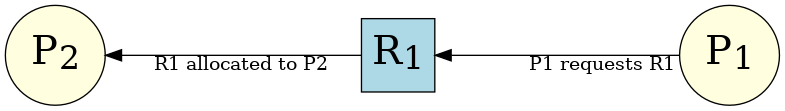
\includegraphics[scale = 0.5]{images/resourceAllocationGraph.png}
\end{center}
\begin{examplebox}{}{}
    A system has m = 2 resources, R1 and R2, and n = 2 processes, P1 and P2.
    \begin{itemize}
        \item P1 has been allocated R1, and is requesting R2.
        \item P2 has been allocated R2, and is requesting R1.
    \end{itemize}
    Draw the resource allocation graph for the scenario. Does the system reach deadlock?
\end{examplebox}
\begin{examplebox}{}{}A system has m = 2 resources, R1 and R2, and n = 2 processes, P1 and P2.
    \begin{itemize}
        \item P1 is requesting R1.
        \item P2 has been allocated R2, and is requesting R1.
    \end{itemize}

    Draw the resource allocation graph for the scenario. Does the system reach deadlock?
\end{examplebox}
\begin{examplebox}{}{}
    Consider the Resource Allocation Graph below. Does it represents a deadlocked state?
    \begin{center}
        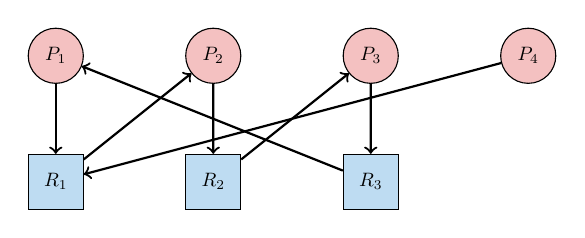
\begin{tikzpicture}[node distance=2cm, every node/.style={scale=0.7}, scale= 0.8]
            % Styles
            \tikzstyle{process} = [circle, draw=black, fill=custom_red!30, minimum size=1cm]
            \tikzstyle{resource} = [rectangle, draw=black, fill=custom_blue!30, minimum width=1cm, minimum height=1cm]

            % Nodes: Processes
            \node[process] (P1) at (0,2) {$P_1$};
            \node[process] (P2) at (2.5,2) {$P_2$};
            \node[process] (P3) at (5,2) {$P_3$};
            \node[process] (P4) at (7.5,2) {$P_4$};

            % Nodes: Resources
            \node[resource] (R1) at (0,0) {$R_1$};
            \node[resource] (R2) at (2.5,0) {$R_2$};
            \node[resource] (R3) at (5,0) {$R_3$};

            % Request edges: Pi → Ri
            \draw[->, thick] (P1) -- (R1);
            \draw[->, thick] (P2) -- (R2);
            \draw[->, thick] (P3) -- (R3);
            \draw[->, thick] (P4) -- (R1);

            % Allocation edges: Ri → Pj
            \draw[->, thick] (R1) -- (P2);
            \draw[->, thick] (R2) -- (P3);
            \draw[->, thick] (R3) -- (P1);
        \end{tikzpicture}
    \end{center}

\end{examplebox}
\begin{itemize}
    \item If there are no cycles, there is no deadlock
    \item If there is deadlock, there must be a cycle
    \item If there is a cycle, there may be deadlock
    \item If each resource has only one instance, and there is a cycle, then
\end{itemize}
\subsection{The Dining Philosophers}
Starvation occurs when a particular process is always waiting for a particular semaphore to become available. \\
The ideas of Deadlock and Starvation are exhibited in the classic synchronization problem: The Dining Philosophers Problem.
\begin{itemize}
    \item There are five philosophers seated at a round table.
    \item Each has a bowl of rice in front of them and a chopstick to their left and right.
    \item They spend their day alternating between eating and thinking.
    \item However there are only five chopsticks...
\end{itemize}

\begin{minipage}{0.48\textwidth}
    If a philosopher is hungry, they will try to pick up the chopstick to the left and then the chopstick to the right. If they manages to do this they will eat for a while before putting down both and thinking for a while. However, if they pick up one, they will not let go of it until they can pick up the second and eat.
\end{minipage}
\begin{minipage}{0.48\textwidth}
    \begin{center}
        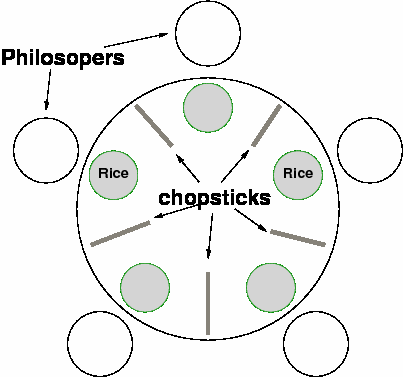
\includegraphics[scale=0.3]{images/diningPhilosophers.png}
    \end{center}
\end{minipage}
Suppose each of the picks up the chopstick to their left. No chopsticks remain on the table so we reach a state of deadlock. The challenge is to find a solution so that.
\begin{itemize}
    \item Deadlock does not occur
    \item Neither does starvation - where one philosopher doesn't eat
\end{itemize}
Recall the “Dining Philosophers Problem” as a model for process synchronisation. For each of the following statements, state if it is true or false, and explain your answer.
\begin{itemize}
    \item If there are five diners, and five chopsticks, and all diners pick up a chopstick at the same time, the system will be in deadlock.
    \item If there are only four diners, and five chopsticks, the system cannot reach a deadlocked state.
    \item If there are six diners, and five chopsticks, the system cannot reach a deadlocked state.
\end{itemize}
In general operating systems take one of three approaches to deal with deadlock:
\begin{itemize}
    \item Ensure that the system will never enter a deadlock state.
    \item Allow the system to enter a deadlock state and then recover.
\end{itemize}
In Case 1, there are two possibilities:
\begin{itemize}
    \item Prevention: we ensure at least one of the four necessary conditions
    \item Deadlock avoidance: where the OS uses a priori information about
\end{itemize}
In Case 2, the OS must have mechanisms for first detecting deadlock and then dealing with it.
Recall that a Semaphore, S, is an integer variable that can only be accessed via one of two operations:
\begin{itemize}
    \item Test/sem\_wait P(S), and
    \item Increment/sem\_post, V(S)
\end{itemize}
It is “special” in the sense that the two operations on it can't be interrupted.
In Lab 6, we will implement a solution to a Race Condition when we have multiple fork'ed subprocesses, problem by implementing a semaphore via a pipe. However, POSIX systems already come with a semaphore solution when working with pthreads. To use it:
\begin{itemize}
    \item sem\_t S; declares S to be a semaphore.
    \item sem\_init(\&S, 0, 1);
    \item sem\_wait(\&S) checks if it is available and, if it is, grabs it.
    \item sem\_post(\&S) releases it, causing awaiting thread to wake up and try taking it.
\end{itemize}
\subsection{Deadlock Detection}
Detection of deadlock is an important, but difficult problem. Using ideas like the Resource Allocation Graph, the system's needs can be represented mathematically, and then a deadlock state checked for\\[2ex]
\textbf{Idea}
Suppose that a system has n processes, and a total of m resources that it can allocate. Resources can only be requested or released one at a time. Then the system is Deadlock free if the following conditions hold:
\begin{itemize}
    \item each process requires at least 1 resource and at most m.
    \item the sum of all their requirements is less than m + n.
\end{itemize}
\subsection{Deadlock Avoidance}
\textbf{Banker's Algorithm} \\
Only allocate resources to a process if you can allocate all the resources it requests. In particular we need to know:
\begin{itemize}
    \item The number of resources the system has.
    \item The number currently allocated to each process;
    \item The maximum that any process might request.
\end{itemize}
With this information, it should be possible to ensure that a circular wait condition does not hold. To understand this, we need to concepts of safe states and safe sequences.
\begin{itemize}
    \item A resources-allocation state is the number of available and allocated resources, and the maximum demands of processes.
    \item A state is safe if the system can allocate resources to each process (eventually), and still avoid deadlock.
    \item A safe sequence is a sequence of processes such that their resource requests can be granted, in order, with no process having to wait indefinitely.
\end{itemize}
\textbf{Example} \\
Suppose we have a system with
\begin{itemize}
    \item three resource types, A, B and C. There are in total 10 instances of
    \item  5 processes, P0 , P1, . . . , P4.
\end{itemize}
\begin{table}[h!]
    \centering
    \begin{tabular}{c|ccc|ccc}
        \hline
        \multicolumn{1}{c}{} & \multicolumn{3}{c|}{\textbf{Total Reqs}} & \multicolumn{3}{c}{\textbf{Current Alloc}}                 \\
        \hline
                             & A                                        & B                                          & C & A & B & C \\
        \hline
        $P_0$                & 7                                        & 5                                          & 3 & 0 & 1 & 0 \\
        $P_1$                & 3                                        & 2                                          & 2 & 2 & 0 & 0 \\
        $P_2$                & 9                                        & 0                                          & 2 & 3 & 0 & 2 \\
        $P_3$                & 2                                        & 2                                          & 2 & 2 & 1 & 1 \\
        $P_4$                & 4                                        & 3                                          & 3 & 0 & 0 & 2 \\
        \hline
    \end{tabular}
    \caption{Resource Allocation Table}
    \label{tab:resource_allocation}
\end{table}



\subsection{Memory Management}

\subsubsection{Summary of main ideas}
\begin{itemize}
    \item "Storage" is how/where long-term data is maintained, particularly while a program is not running.
    \item During execution, a program (now, a process) has data stored in main memory, also known as "primary storage".
    \item Data belonging to a process is stored in "actual" memory: integrated circuits physically located on the device.
    \item The OS presents this location to the device as a logical address.
    \item The OS can use (backing) storage as temporary main memory, using "swapping".
\end{itemize}

\subsection{Memory and Storage Management}
So far, in the "OS" component of CS211 we have focused on:
\begin{itemize}
    \item OS Structure
    \item Processes - what are they?
    \item Process scheduling (w.r.t. CPU time)
    \item Process resource allocation.
\end{itemize}

We didn't really discuss what these "resources" are. In this final section of CS211 we will look at the management of the most important resources (other than CPU time): memory and storage.

In the textbook (OSTEP),
\begin{itemize}
    \item Memory is covered Chapters 13-23 (which shows that we don't do it in full detail here), as part of Virtualisation.
    \item Storage is covered in Chapters 36-50, under the heading of Persistence. Unfortunately, along with security, it is largely omitted from CS211.
\end{itemize}

Roughly, "storage" refers to how long-term data is maintained, particularly while a program is not running. Traditionally, this was on disks (drives), more recently it is on networked (cloud) devices.

But during execution, a program (now, a process) has data stored in main memory.

Management of both main memory and long-term storage require a high degree of sophistication on the part of the operating system.

This section consists of:
\begin{itemize}
    \item Memory Management
    \item Virtual Memory
    \item Programming with memory addresses (pointers).
\end{itemize}

A program must be brought into (main) memory and placed within a process for it to be executed. An Input queue is maintained, i.e., a collection of jobs on the disk that are waiting to be brought into memory for execution. User programs go through several steps before being executed, in particular they must be allocated space in memory.

Furthermore, recalling CPU Scheduling: the OS attempts to maximise CPU usage and responsiveness by switching between processes. This means that memory must be allocated to a (possibly large) number of processes at any given time.

This leads to several complications:
\begin{enumerate}
    \item Since there are many processes running, the OS must have a fair way of allocating memory to all running processes.
    \item As we've seen with fork()'ed processes, two processes can think they have access to the same memory address. So some virtualization is needed.
    \item Most computers have different types of "memory", such as cache, RAM, and backing storage. The OS presents a single coherent view of all this to processes.
    \item Physical memory is not necessarily large enough to accommodate all the processes, and so secondary storage must be used as "over-flow" memory.
\end{enumerate}

A logical address is generated by the CPU; The OS uses this address. It is also referred to as a virtual address. A physical address is that what is used by the memory unit, i.e., the one loaded into the memory address register.

The OS takes care of mapping between the logical addresses and the physical addresses.

The virtual address is unique within a process. That is, no two variables belonging to a process can be stored at the same virtual address.

But two different processes could use the same virtual address.

You can check the virtual address used by a C program as follows:

\begin{lstlisting}[language=C]
int x;
fork(); // Now there are 2 processes.
x = getppid();
printf("[%d] x stores the value %d at %p\n",
    getpid(), x, &x);
\end{lstlisting}

The output I get is:
\begin{verbatim}
x is stores 21106 at 0x7fff1650fdc4
x is stores 21107 at 0x7fff1650fdc4
\end{verbatim}

\subsection{Contiguous Memory Allocation}
In a multiprogramming environment, memory space is occupied by the operating system and a collection of user processes.

In order to maximise the degree of multiprogramming on the system, the OS will load as many processes into memory as there is space for.

When new processes arrive in the input queue, it picks the first one and loads it into memory unless there is not enough room to accommodate it ("Banker's Algorithm").

In this case, it may search through to processes in the Input queue and load the first one for which there is a large enough space to accommodate.

When user processes terminate, memory "holes" are created. The operating system must allocate one of these holes to a new process that is starting.

If the hole is too large, only part of it is allocated and a new smaller hole is created. Also, when a process terminates, if its space is adjacent to a free hole, they are amalgamated to create a larger one.

The scheduler then checks if the new hole is large enough to accommodate the next job in the Input queue.

Analogy: books in a book-case (where we can't change the position of any book on the case)

If this procedure of splitting and amalgamating of holes continues for a while, we end up with blocks of available memory of various sizes scattered throughout memory. This is called Fragmentation and is to be avoided.

Strategies/Algorithms for allocating memory to processes is a crucial part of memory management.

Three different strategies (see Section 17.3) are:
\begin{enumerate}
    \item First Fit (FF): allocate the first hole that is large enough to accommodate the new process. This is the fastest method, but may cause the most fragmentation-i.e., the most small "pockets" of unused non-contiguous memory.
    \item Best Fit (BF): search all available holes and allocate the smallest hole that is big enough to accommodate the new process. This is slower than best-fit, but leads to the smallest "pocket" sizes.
    \item Worst Fit (WF): search all available holes and assign part of the largest available hole. This is the slowest method but may leave a smaller number of larger holes than either first or best fit.
\end{enumerate}

\subsection{Example}
Suppose that a system has four free memory holes ordered as follows:

\[
    H_{1}=100 \mathrm{k}, H_{2}=500 \mathrm{k}, H_{3}=200 \mathrm{k}, H_{4}=300 \mathrm{k}
\]

Four jobs (i.e., processes) requiring (contiguous) memory space of various sizes are submitted at the same time in the order given below.

\begin{tabular}{|c|c|c|c|c|}
    \hline
    Process & $P_{1}$ & $P_{2}$ & $P_{3}$ & $P_{4}$ \\
    \hline
    Size    & 140 k   & 450 k   & 200 k   & 300 k   \\
    \hline
\end{tabular}

Show how these would be allocated by the FF and BF strategies.

\begin{tabular}{|c|c|c|c|c|}
    \hline
    Process & $P_{1}$ & $P_{2}$ & $P_{3}$ & $P_{4}$ \\
    \hline
    Size    & 140 k   & 450 k   & 200 k   & 300 k   \\
    \hline
\end{tabular}

\subsubsection{First Fit}

\begin{tabular}{|c|c|c|c|}
    \hline
    $H_{1}(100)$ & $H_{2}(500)$ & $H_{3}(200)$ & $H_{4}(300)$ \\
    \hline
                 &              &              &              \\
    \hline
\end{tabular}

\subsubsection{Best Fit}

\begin{tabular}{|c|c|c|c|}
    \hline
    $H_{1}(100)$ & $H_{2}(500)$ & $H_{3}(200)$ & $H_{4}(300)$ \\
    \hline
                 &              &              &              \\
    \hline
\end{tabular}

\begin{tabular}{|c|c|c|c|c|}
    \hline
    Process & $P_{1}$ & $P_{2}$ & $P_{3}$ & $P_{4}$ \\
    \hline
    Size    & 140 k   & 450 k   & 200 k   & 300 k   \\
    \hline
\end{tabular}

\subsubsection{Worst Fit}

\begin{tabular}{|c|c|c|c|}
    \hline
    $H_{1}(100)$ & $H_{2}(500)$ & $H_{3}(200)$ & $H_{4}(300)$ \\
    \hline
                 &              &              &              \\
    \hline
\end{tabular}

Memory is partitioned into contiguous segments and allocated to different processes. The methods for contiguous memory allocation described above can lead to:
\begin{itemize}
    \item External fragmentation: total memory space exists to satisfy a request, but it is not contiguous. That is, memory is available but is broken up into "pockets" between partitions that are too small to be used.
    \item Internal fragmentation: Suppose there is a free hole of size 12,100 bytes and we require a partition of size 12,080 bytes. The OS may require more than 20 bytes to keep track of the unused portion, so it can be more economical to allocate all 12,100 bytes even though this is slightly larger than requested memory; this is called "internal fragmentation".
\end{itemize}

\subsection{Paging}


\subsection{Basic idea}
\begin{itemize}
    \item Logical address space of a process can be non-contiguous; process is allocated physical memory whenever the latter is available ("chop up the processes").
    \item Divide physical memory into fixed-sized blocks called frames. All frames on the system are of the same size, usually some power of 2, determined by the hardware ("chop up the space").
\end{itemize}

To find out the page size on a Linux system, run this program:

\begin{lstlisting}[language=C]
#include <stdio.h>
#include <unistd.h> /* sysconf(3) */
int main(void) {
    printf("The page size for this system is %ld bytes.\n",
        sysconf(_SC_PAGESIZE)); /* _SC_PAGE_SIZE is OK too. */
    return 0;
}
\end{lstlisting}

The output I get when running this is:
\begin{verbatim}
The page size for this system is 4096 bytes.
\end{verbatim}

\subsection{Try this on a Windows system}

\begin{lstlisting}[language=C]
#include <stdio.h>
#include <windows.h>
int main(void) {
    SYSTEM_INFO si;
    GetSystemInfo(&si);
    printf("The page size for this system is %u bytes.\n", si.dwPageSize);
    return 0;
}
\end{lstlisting}

What output do you get?

\begin{itemize}
    \item Logical memory into blocks called pages.
    \item Frames and Pages are of the same size.
    \item The OS keeps track of all free frames in memory.
    \item To run a program that will use $n$ pages, we need to find $n$ free frames and load the program.
    \item Page Table maintained to translate logical to physical addresses.
\end{itemize}

\subsection{Address Translation Scheme}
An address generated by CPU is divided into:
\begin{itemize}
    \item Page number ($p$), used as an index into a page table which contains the base address of each page in physical memory.
    \item Page offset ($d$), combined with the base address to define the physical memory address that is sent to the memory unit.
\end{itemize}


\subsection{Basic ideas}
\begin{itemize}
    \item Bring a page into memory only when it is needed (lazy paging).
    \item Pages belonging to a process may be memory resident or not.
    \item The system needs some mechanism for distinguishing between resident and non-resident pages. Therefore the page table associates a valid/invalid bit with each page.
    \item $1 \Rightarrow$ valid/resident \quad $0 \Rightarrow$ invalid/not in physical memory.
    \item If a process wishes to access a valid page (a "HIT") it can do so.
    \item If a process wishes to access an invalid page (a "MISS") then the paging hardware generates a Page Fault.
\end{itemize}

If there is a reference to an invalid page, reference will trap to OS.
\begin{itemize}
    \item Reference to nonexisting page $\rightarrow$ abort
    \item Just not in memory $\rightarrow$ must bring page into memory.
\end{itemize}

\begin{enumerate}
    \item Reference is made to invalid page
    \item Page fault generated - call to Operating system.
    \item Locate empty frame in physical memory.
    \item Swap page into frame.
    \item Reset tables, flip validation bit (change to 1)
    \item Restart user process.
\end{enumerate}

Of course, this assumes that there is an empty frame in memory...

\subsection{What happens if there is no free frame?}
\subsubsection{Page replacement}
Find some page in memory that is not in use, and swap it out. We need an algorithm for selecting such a page. The algorithm will be evaluated on the basis of the generation of a minimum number of page faults.

Page fault handling is slow, so the performance of the whole system depends heavily on having an efficient Page Replacement algorithm - one with the lowest possible page fault rate.

To evaluate a page replacement algorithm, we will consider:
\begin{itemize}
    \item An example where a program has the following stream of virtual pages (also called the "page reference string")
\end{itemize}

\[
    \{1,2,3,4,1,2,5,1,2,3,4,5\}
\]

This means it first references page \#1, then page \#2, then page \#3,... finally page \#5. ...

\begin{itemize}
    \item $F$, the number of frames on the system
    \item the algorithm.
\end{itemize}

For these we shall compute the Frame Hit Rate:

\[
    \frac{\text{number of Hits}}{\text{Length of page reference string}}
\]

The greater the hit rate, the better.

When a free frame is needed, the victim is the page that has been in memory the longest.
Suppose that $F=3$, and that at the start no pages are in memory. Then we get

\begin{tabular}{|c|c|c|c|c|c|c|c|c|c|c|c|c|}
    \hline
    1    & 2    & 3    & 4    & 1    & 2 & 5 & 1 & 2 & 3 & 4 & 5 \\
    \hline
    MISS & MISS & MISS & MISS & MISS &   &   &   &   &   &   &   \\
    \hline
    1    & 2    & 3    &      &      &   &   &   &   &   &   &   \\
    \hline
         & 1    & 2    &      &      &   &   &   &   &   &   &   \\
    \hline
         &      & 1    &      &      &   &   &   &   &   &   &   \\
    \hline
\end{tabular}

If we wanted to improve the hit rate, we could try increasing the number of frames. So, let's redo the previous example, but with $F=4$.

\begin{tabular}{|c|c|c|c|c|c|c|c|c|c|c|c|c|}
    \hline
    1    & 2    & 3    & 4    & 1 & 2 & 5 & 1 & 2 & 3 & 4 & 5 \\
    \hline
    MISS & MISS & MISS & MISS &   &   &   &   &   &   &   &   \\
    \hline
    1    & 2    & 3    & 4    &   &   &   &   &   &   &   &   \\
    \hline
         & 1    & 2    & 3    &   &   &   &   &   &   &   &   \\
    \hline
         &      & 1    & 2    &   &   &   &   &   &   &   &   \\
    \hline
         &      &      & 1    &   &   &   &   &   &   &   &   \\
    \hline
\end{tabular}

This is called Bélady's Anomaly: sometimes increasing the number of frames can increase the number of page faults!

Optimal algorithm requires the least number of page faults and does not suffer for Belady's Anomaly: Replace page that will not be used for longest period of time. However, one needs to know what pages will be referenced in the future. So this is difficult to implement.

LRU: The Least Recently Used (LRU) algorithm is similar to FIFO but, rather than removing the frame that has been in memory the longest, we remove the one that has not been referenced for the longest time.

\subsection{Exercise}
Re-do the examples from Slides 26 and 27. How many Page faults are generated?

\subsection{Memory management in C}
We'll finish with a short note about how a process can request memory from the OS. We'll need to recall, from Week 4 (Part 2):

\begin{itemize}
    \item A Pointer is a special variable that has as its value a memory location.
    \item Declaring a pointer to an integer is done by:
          \begin{verbatim}
    int *p;
    \end{verbatim}
    \item The variable $p$ can contain an address.
    \item Access the contents of that address with $*p$.
\end{itemize}

In this context, the $*$ symbol is called a dereferencer.

It is reasonable to think of \& as the inverse of the operator $*$. This is because \&i means "the address of the variable stored in i", while *p means "the value stored at the address $p$.

If $i$ is an integer with value 23 then
\begin{verbatim}
*(&i)
\end{verbatim}
will evaluate as 23. However,
\begin{verbatim}
&(*i)
\end{verbatim}
is illegal. Why?

If we declare $p$ as a pointer to an integer and set
\begin{verbatim}
p = &i;
\end{verbatim}
then
\begin{verbatim}
&(*p)
\end{verbatim}
will evaluate as the address of $i$.

Question: Is $*(\&p)$ legal? If so, what will it evaluate as?

When an array of integers is declared, e.g.,
\begin{verbatim}
int a[10];
\end{verbatim}
what actually happens is:
\begin{itemize}
    \item The system declares a pointer to an integer called $a$.
    \item The pointer is to $a[0]$, the "base address" of the array.
    \item Space is allocated to the addresses pointed to by $a, a+1, \ldots, a+9$.
\end{itemize}

It is not true that arrays and pointers are exactly the same. If we declare:
\begin{verbatim}
int *p, a[10];
\end{verbatim}
the value of the pointer $p$ can be reassigned anytime we like, but the value of $a$ is fixed.

However, because of this, we use pointers when we wish to pass arrays as functions.

Here is an example of passing an array as an argument to a function.

Given an integer array $a$, we’ll calculate $\sum_{i=0}^{n} a_{i}$.

\begin{lstlisting}[language=C]
int sum_pointer(int *p, int n);
int sum_array(int a[], int n);

int main()
{
    int a[4] = {1, 99, 40, 60};
    printf("a[0]+a[1]+a[2]=%d\n", sum_array(a,3));
    printf("a[1]+a[2]+a[3]=%d\n", sum_pointer(a+1,3));
    return(0);
}

int sum_pointer(int *p, int n)
{
    int i, sum=0;
    for (i=0; i<n; i++)
        sum+=*(p+i);
    return(sum);
}

int sum_array(int a[], int n)
{
    int i, sum=0;
    for (i=0; i<n; i++)
        sum+=a[i];
    return(sum);
}
\end{lstlisting}

Before studying dynamic memory allocation, we will work out how much storage is required by integers, floats, characters, and even pointers. This is because we need to tell the system how many bytes are required to store an array. Although we can hard-code this into our program, we prefer not to since:
\begin{itemize}
    \item We might make a mistake.
    \item Some systems store data types differently from others (standards for the C language specify the minimum number of bytes used, but this can be exceeded).
    \item There are more complex structures which have variable memory requirements.
\end{itemize}

So we use the \texttt{sizeof()} operator. (Note: you've already seen this when using the read and write functions for pipes).

The \texttt{sizeof()} operator returns the number of bytes for a particular data type.

It can take data types (e.g., float, char) or variable names as its argument.

It returns an unsigned integer.

\begin{lstlisting}[language=C]
int x=-123, *p; char name[6]="CS211";
printf("A char takes\t\t %3lu bytes;\n", sizeof(char));
printf("A float uses\t\t %3lu bytes;\n", sizeof(float));
printf("A double uses\t\t %3lu bytes;\n", sizeof(double));
printf("x is requires\t\t %3lu bytes;\n", sizeof(x));
printf("A pointer needs\t\t %3lu bytes;\n", sizeof(p));
printf("Array %s is stored in %3lu bytes;\n", name, sizeof(name));
printf("enum MONTH takes\t %3lu bytes;\n", sizeof(MONTH));
printf("struct Date takes\t %3lu bytes.\n", sizeof(Date));
\end{lstlisting}

The output I get is:

\begin{tabular}{|c|c|}
    \hline
    A char takes             & 1 bytes;  \\
    \hline
    A float uses             & 4 bytes;  \\
    \hline
    A double uses            & 8 bytes;  \\
    \hline
    x is requires            & 4 bytes;  \\
    \hline
    A pointer needs          & 8 bytes;  \\
    \hline
    Array CS211 is stored in & 6 bytes;  \\
    \hline
    enum MONTH takes         & 4 bytes;  \\
    \hline
    struct Date takes        & 12 bytes. \\
    \hline
\end{tabular}

\subsection{Dynamic memory allocation}
Having to declare the size of an array in a function header is a huge restriction. Either we have to modify the program every time we change the size of the array, or we have to define the array to be as big as possible.

This is wasteful of time and resources.
To minimize the amount of coding we have to do, and to use resources well, we simply declare an appropriate variable with type:
\begin{itemize}
    \item Pointer to int for an integer vector: \texttt{int *v}
\end{itemize}

Next we must ask the system to reserve some memory. There are four important commands:
\begin{itemize}
    \item \texttt{sizeof()} (see above)
    \item \texttt{calloc(n, sizeof(x))}: Continuous Memory Allocation. It will reserve enough space to $n$ variables each with the same size as $x$. It sets them all to zero.
    \item \texttt{malloc(n*sizeof(int))}: Memory Allocation. As above, but it doesn't do any initialization.
    \item \texttt{free(ptr)}: deallocate the space that begins at the address stored in \texttt{ptr}.
\end{itemize}

The headers for these functions are in \texttt{stdlib.h}.

The important thing is that we can call \texttt{calloc()}, \texttt{malloc()}, and \texttt{free()} any time we like. This is what is dynamic about it.

Both \texttt{malloc()} and \texttt{calloc()} return pointers to the base of the memory they allocated. However, because they are not for specific pointer types (e.g., pointer to int or pointer to char) they return "void pointers".

These 'void pointers' are then automatically promoted to the relevant pointer type, so the following is correct:

\begin{lstlisting}[language=C]
int c;
float x;
c = malloc(7*sizeof(char));
x = calloc(10, sizeof(float));
\end{lstlisting}

In the example below, the size of the vector $v$ is not fixed until the program is run. Note that the sum function will work for any sized array.

\begin{lstlisting}[language=C]
int main(void)
{
    int *v, n, i, ans;
    printf("How many elements are there in v? :");
    scanf("%d", &n);
    v = (int *)calloc(n, sizeof(int));
    for (i=0; i < n; i++)
    {
        printf("Enter v[%d]: ", i);
        scanf("%d", &v[i]);
    }
    ans = sum(v, n);
    printf("The sum of the entries of v is %d \n", ans);
    free(v);
    return(0);
}
\end{lstlisting}

\section{Module Review}

The topics we have covered (not necessarily in order) are:
\begin{enumerate}
    \item What is an OS?
    \item Computer History: from batch systems to distributed systems.
    \item Programming with processes: fork(), getpid(), ...
    \item Interprocess communication with pipe(), kill(), signal()
    \item Threads, including pthreads
    \item Process Scheduling Algorithms.
    \item Concurrency; race conditions; Critical Sections; locks; Semaphores;
    \item The dining Philosophers problem
    \item Resource allocation; Banker's algorithm.
    \item Memory management; Contiguous allocation;
    \item Pages and frames; Page replacement algorithms.
\end{enumerate}

In C Programming, we had:
\begin{enumerate}
    \item Basic structure. Comments. Header files.
    \item Key-words and operators.
    \item Selection statements: if else, etc. Logic operators.
    \item Loops: for, while, do... while;
    \item Input (printf()) and output scanf(); conversion characters.
    \item Functions, including argument lists, return values, void, call-by-value; call-by-reference.
    \item Pointers
    \item Multidimensional arrays; strings, and all the str* functions.
    \item Files: fopen(), fclose(), reading and writing; navigating
    \item User-defined types enum, struct, typedef
    \item Dynamic memory allocation: calloc(), malloc(), free()
\end{enumerate}

\section*{Q2 (f)}

Which of the following CPU scheduling algorithms are preemptive? Select all that apply.
\begin{enumerate}
    \item First Come First Served (FCFS),
    \item Shortest Job First (SJF),
    \item Shortest Time To Completion First (STCF),
    \item Round Robin (RR).
\end{enumerate}

The table below shows the CPU burst times (in seconds) of four processes submitted in the given order, all at time $t=0$.

\begin{tabular}{ccccc}
    \toprule
    Process    & $P_{1}$ & $P_{2}$ & $P_{3}$ & $P_{4}$ \\
    \midrule
    Burst Time & 20      & 10      & 15      & 5       \\
    \bottomrule
\end{tabular}

Sketch Gantt charts for how these processes are scheduled for each of the following algorithms.
\begin{enumerate}
    \item First-Come-First-Served (FCFS),
    \item Shortest-Job-First (SFJ), and
    \item Round Robin with a time quantum of $q=5$ seconds
\end{enumerate}

You may assume that context switching is instantaneous. Calculate the average turn-around and response times for each algorithm.

\subsection*{FCFS}

\subsection*{SJF}

\subsection*{RR}

\section*{Q3 (f)}

What is a Resource Allocation Graph? Explain the relation between cycles in the graph and system deadlock in the case where there is a single instance of each resource.

Consider the two Resource Allocation Graphs in Figure~\ref{fig:resource_allocation}. In both scenarios presented there are four processes, $P_{1}, P_{2}, P_{3}$ and $P_{4}$, and three resources, $R_{1}, R_{2}$, and $R_{3}$, of which there is one instance each.
\begin{enumerate}
    \item Determine if it represents a deadlocked state.
    \item If it is deadlocked, explain why.
    \item If it is not deadlocked, explain how the resource allocation would proceed so that, eventually, all processes received their desired resource allocation. (You may assume that if a process has its desired resource allocation it will eventually terminate and release that allocation).
\end{enumerate}



Suppose a system has three running processes, each of which requires three resources of a particular type. Furthermore the system has five instances of that resource. Explain, with the aid of a resource allocation graph, how the system could reach deadlock.

Suppose a system has two free memory partitions, of size 400 k and 600 k, in that order.

Four jobs requiring (contiguous) memory space of various sizes are submitted at the same time, and in the following order:

\begin{tabular}{ccc}
    \toprule
    Process & Order submitted & Size  \\
    \midrule
    $P_{1}$ & 1st             & 320 k \\
    $P_{2}$ & 2nd             & 200 k \\
    $P_{3}$ & 3rd             & 280 k \\
    $P_{4}$ & 4th             & 200 k \\
    \bottomrule
\end{tabular}

\begin{enumerate}
    \item Would all these processes be allocated memory if the First-Fit (FF) scheme is employed? If not, which one(s) would be omitted?
    \item Would all these processes be allocated memory if the Worst-Fit (WF) scheme is employed? If not, which one(s) would be omitted?
\end{enumerate}

\subsection*{First Fit}

Holes: 400k, 600k. Requests: 320k, 200k, 280k, 200k

Holes: 400k, 600k. Requests: 320k, 200k, 280k, 200k

Suppose a system has $F=4$ available frames, and executes a process that has the following "page reference string"

\[
    \{1,2,3,1,4,5,1,4,2,4,3,4\}
\]

\begin{enumerate}
    \item Calculate the Frame Hit rate using the First-In-First-Out algorithm.
    \item Calculate the Frame Hit rate using the Least Recently Used algorithm.
    \item What would be Frame Hit rate be for both these algorithms if we increase the number of frames (i.e., $F \geq 5$)?
\end{enumerate}

\[
    \{1,2,3,1,4,5,1,4,2,4,3,4\}
\]

\subsection*{Five or more frames}

\[
    \{1,2,3,1,4,5,1,4,2,4,3,4\}
\]
\end{document}